\documentclass[pdflatex,sn-mathphys-num]{sn-jnl}

\usepackage{graphicx}
\usepackage{listings}
\usepackage{xcolor}
\usepackage{booktabs}
\usepackage{float}
\usepackage{caption}
\usepackage{subcaption}
\usepackage{amsmath}
\usepackage{tcolorbox}
\usepackage{lipsum}
\usepackage{multirow}
\usepackage{mathrsfs}
\usepackage{amssymb}
\usepackage{algorithm}
\usepackage{algpseudocode}

\begin{document}

\title{Assignment 1 - Crowdfunding Company}

\author*[1]{\fnm{Carlo} \sur{Falchi}}\email{carlo.falchi@studenti.unimi.it}
\author*[1]{\fnm{Francesco} \sur{}}\email{francesco.palladini@studenti.unimi.it}
\affil[1]{\orgdiv{Department of Computer Science}, \orgname{University of Milan}, \country{Italy}}

\maketitle
\begin{figure}[ht]
    \centering
    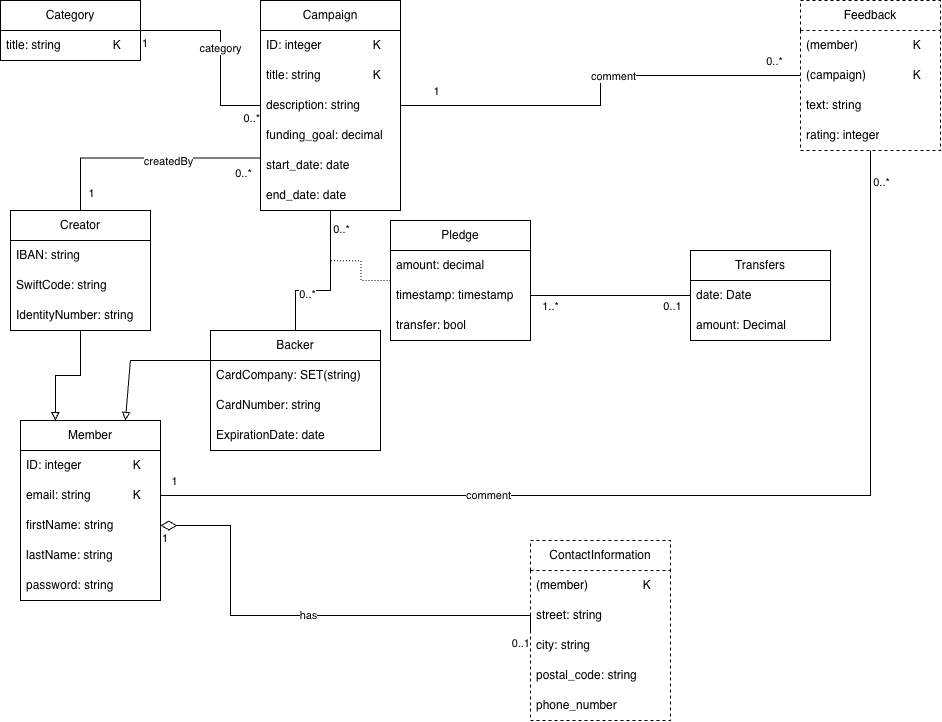
\includegraphics[width=0.9\textwidth]{uml/uml.png}
    \caption{UML Diagram}
     \label{fig:uml}
\end{figure}
\section{Solution}

\subsection{Assumption}
\subsection{Constraints}
\subsection{Workload}
\begin{figure}[ht]
    \centering
    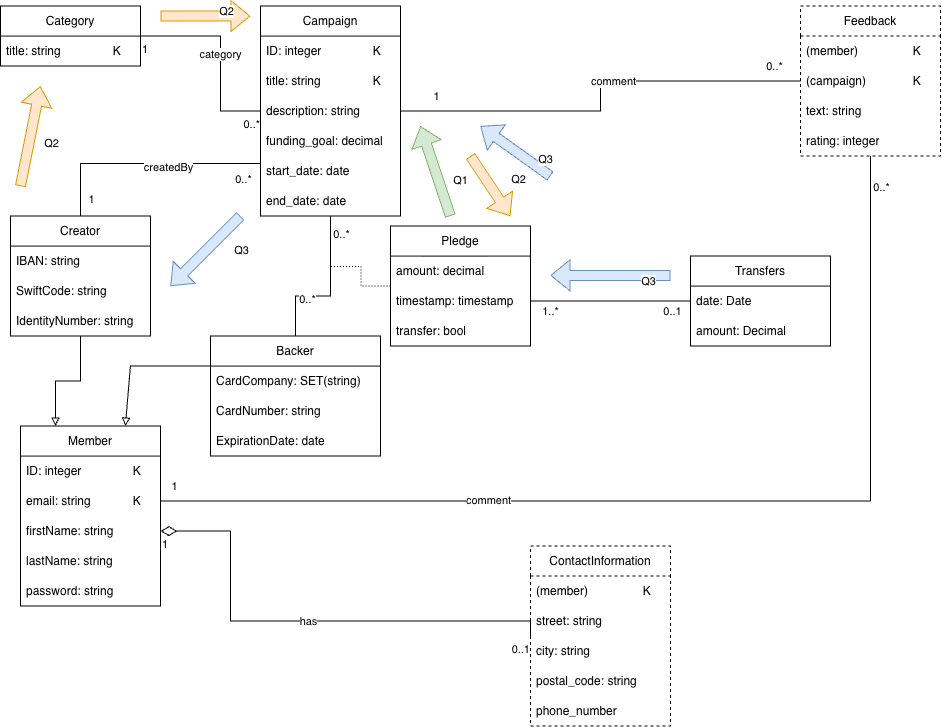
\includegraphics[width=0.9\textwidth]{uml/workload.png}
    \caption{Representation Workload}
     \label{fig:workload}
\end{figure}
\end{document}